\section{Ejercicio 01: } 

El siguiente diagrama E / R simplificado describe el envío de mercancías. Los lotes pertenecientes a ciertos grupos se
envían a ciertos destinos en varios países a través de diferentes modos de transporte. Un cierto centro de costos es
responsable de cada envío. La dimensión de tiempo consiste en mes y año.

	\begin{center}
	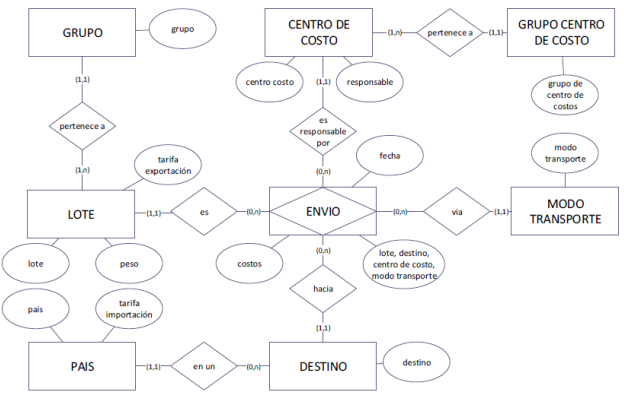
\includegraphics[width=18cm]{./Imagenes/1}
	\end{center}	

Supongamos que los costos de los atributos ya incluyen todas las tarifas. No se transferirá más información sobre las tarifas
al almacén de datos. El análisis tendrá lugar a nivel del grupo de centros de costos, no se necesita información sobre los
centros de costos.
Por favor identifique el hecho de interés y construya el Modelo Dimensional y su respectivo diagrama físico

DESARROLLO 
EJERCICIO 01

	\begin{center}
	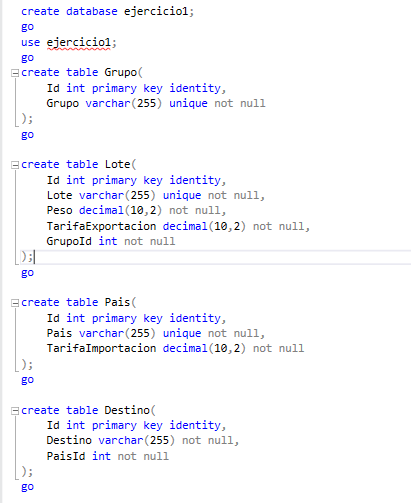
\includegraphics[width=17cm]{./Imagenes/11}
	\end{center}

	\begin{center}
	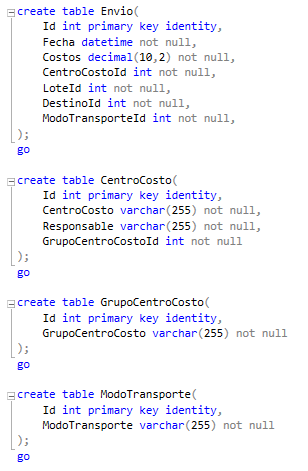
\includegraphics[width=17cm]{./Imagenes/12}
	\end{center}

	\begin{center}
	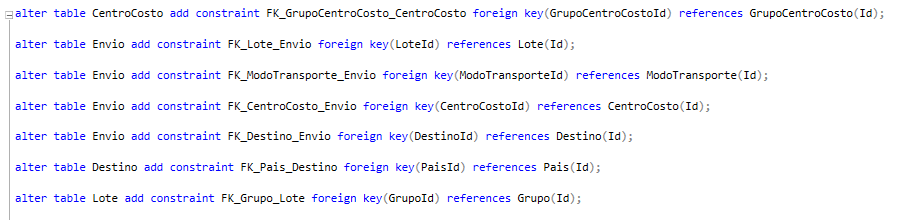
\includegraphics[width=17cm]{./Imagenes/13}
	\end{center}

MODELO DIMENSION 01

	\begin{center}
	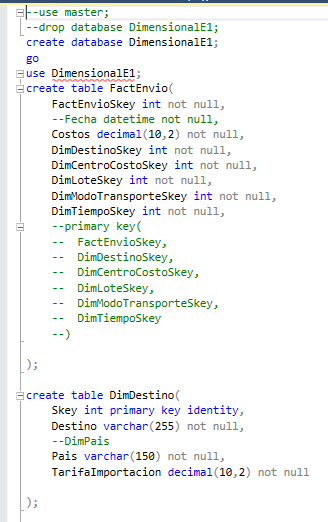
\includegraphics[width=17cm]{./Imagenes/14}
	\end{center}

	\begin{center}
	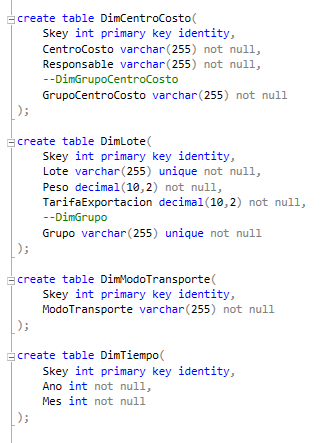
\includegraphics[width=17cm]{./Imagenes/15}
	\end{center}

	\begin{center}
	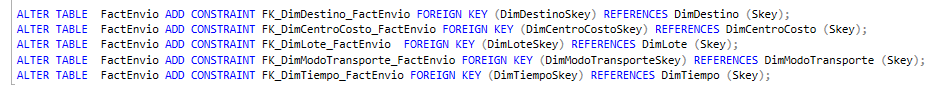
\includegraphics[width=17cm]{./Imagenes/16}
	\end{center}